\chapter{Step 04: Storing the DIP Switch}
\label{ch:step04}

Step 03 showed a number on the display; now we choose the number ourselves.
The design of \cc{04_dip_switch} reads eight bits from a DIP switch and stores
them in an 8-bit register when the first button is pressed. The display shows
the register. There is almost no new SystemVerilog in this step. What is new is
that a button controls a register, and after the bouncing button at the end
of Chapter~\ref{ch:step02} we look closely at what this means.

\section{The Circuit}
\label{sec:step04-circuit}

A DIP switch is a row of eight small switches, each one giving a constant bit
for as long as we leave it alone. It sits on its own PMOD module, here on
PMOD 1B, next to the display on PMOD 1A (Figure~\ref{fig:step04-board}).

\begin{figure}[ht]
\centering
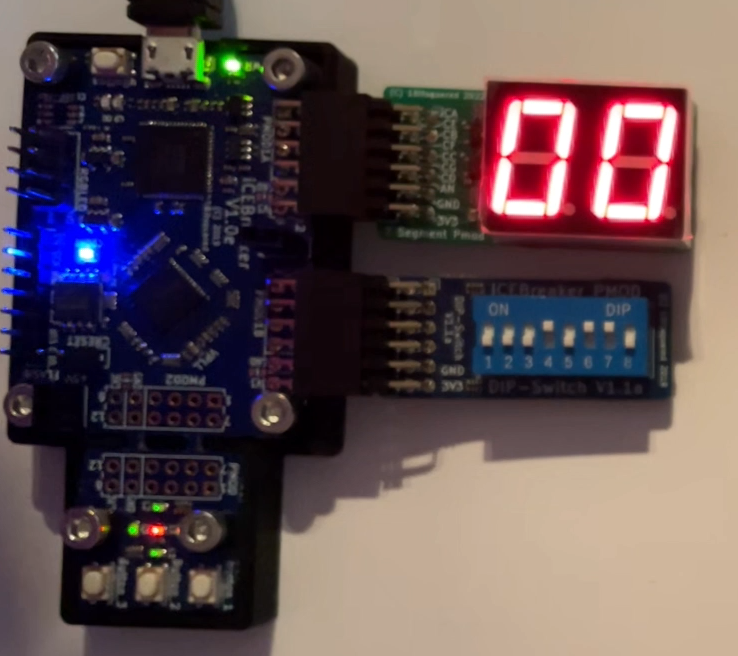
\includegraphics[width=0.55\linewidth]{figures/04_board.png}
\caption{The board with the 7-segment display (PMOD 1A, top right), the DIP
switch (PMOD 1B, right) and the module with buttons and LEDs (PMOD 2,
bottom). The display shows \cc{00}, the power-up value of the register.}
\label{fig:step04-board}
\end{figure}

The circuit is an 8-bit register with enable. Its data inputs are the switches,
its enable is the button:
\[
  \mathit{hex\_val}' =
  \begin{cases}
    \mathit{hex\_in}, & \text{if } \mathit{BTN1} = 1,\\
    \mathit{hex\_val}, & \text{otherwise,}
  \end{cases}
\]
and \cc{dev_hex} from Chapter~\ref{ch:step03} shows \cc{hex_val}.

\section{The Description in SystemVerilog}
\label{sec:step04-sv}

\svfile{04_dip_switch/test.sv}

Every piece of this was introduced in Chapter~\ref{ch:step03}. The file
\cc{dev_hex.sv} in this directory is a link to the one of step 03, so both
steps use the same display driver.

\textbf{The bit order.} Line 26 collects the eight switch inputs into a
vector, with \cc{B0} on the left:
\begin{lstlisting}
assign hex_in = {B0, B1, B2, B3, B4, B5, B6, B7};
\end{lstlisting}
So \cc{B0} is \cc{hex_in[7]}, the most significant bit, and \cc{B7} is
\cc{hex_in[0]}. If \cc{B0} to \cc{B7} are the switches 1 to 8 from left to
right, the switches read as the binary number from left to right, the way we
write numbers. (The concatenation makes this possible without a single gate:
it only decides which wire is which bit.)

\textbf{The register.} The \cc{always_ff} block in lines 30--34 is the
register with enable of Section~\ref{sec:step04-circuit}: \cc{if (BTN1)}
loads, and without an \cc{else} the register keeps its value. This is the
same construction as \cc{hex_val} in step 03, only with \cc{hex_in} instead of
\cc{hex_val + 1}, and with the button instead of \cc{tic}.

\section{What yosys Makes of It}
\label{sec:step04-yosys}

\outputfile{step04_yosys_stat.txt}

Compared with step 03, the one-second counter is gone (no \cc{SB_DFFSR}, 36
fewer \cc{SB_CARRY}), and what is left besides \cc{dev_hex} is the register. Its
eight flip-flops in the netlist:

\outputfile{step04_cells.txt}

This is as direct as it gets. Each switch goes straight into the data input
\cc{D} of a flip-flop, and the button straight into all eight enable inputs
\cc{E}. There is no LUT between them: the multiplexer of the \cc{if} is the
enable of the \cc{SB_DFFE}. (The yosys option \cc{-dffe_min_ce_use 4} in the
Makefile says to use the enable input only if at least four flip-flops share
the same enable signal; for a single flip-flop like \cc{digit_sel} in
\cc{dev_hex}, yosys builds the multiplexer with a LUT instead.)

The flip-flops are clocked by \cc{CLK}, not by the button. This is the
difference to the experiment of Exercise~\ref{ex:step02-button}, where the
button \emph{was} the clock.

\section{The Button}
\label{sec:step04-button}

In Exercise~\ref{ex:step02-button}, the state sometimes advanced by two or more
steps per press, because the contacts of the button bounce: for a few
milliseconds after we press it (and again when we release it), the signal
jumps between 0 and 1 several times. Each of these jumps was a clock edge.

Here, \cc{BTN1} is not a clock. At every edge of the 12\,MHz clock, the
register looks at the button. Pressing it for a tenth of a second means that
\cc{BTN1} is 1 at about 1.2 million clock edges, and at each of them the
register loads the switches. During the bouncing, the enable goes on and off a
few times, and the register loads in some cycles and not in others.

None of this matters, because loading is \emph{idempotent}: loading the same
value twice gives the same result as loading it once. Let $L_s$ be the map
``load $s$'', $L_s(h) = s$ for every register value $h$. Then $L_s \circ L_s =
L_s$, and whether the register loads once, three times or a million times
during a press, it ends up with $s$, the setting of the switches. In step 02
the map applied per edge was the next-state map of the state machine, and
applying it twice is not the same as applying it once. That is why bouncing
mattered there and does not matter here.

\textbf{Is the button synchronised?} No. The button changes whenever we press
it, not in step with the clock, and its signal goes straight into the enable
inputs of eight flip-flops. If it changes just before a clock edge, it may
reach some of the eight flip-flops in time and others not, and in rare cases a
flip-flop may even need a little longer than usual to decide between 0 and 1
(\term{metastability}). Usually one samples such an input with two flip-flops
in a row first, a \term{synchroniser}, and uses only the output of the second
one. Here we can do without: if some flip-flops load at the edge where the
press begins and others do not, they all load at the next edge, 83\,ns later.
And when the button is released, all eight bits already hold the setting of
the switches, so it does not matter which of them load once more.

\begin{exercise}
\label{ex:step04-change}
Press the button, and while you keep it pressed, change a switch. What does
the display do? What happens if you change a switch while the button is not
pressed?
\end{exercise}

\begin{exercise}
\label{ex:step04-count}
Suppose we want to count the presses of \cc{BTN1} instead: \cc{hex_val} is
incremented by one per press. Why does \cc{if (BTN1) hex_val <= hex_val + 1;}
not work? Describe a circuit that produces a pulse of one clock cycle when
the (synchronised) button changes from 0 to 1, write it in SystemVerilog, and
say what bouncing does to it.
\end{exercise}

\section{What nextpnr Makes of It}
\label{sec:step04-pnr}

\outputfile{step04_pnr_util.txt}

29 logic cells: the eight flip-flops of the register and \cc{dev_hex}.
18 \cc{SB_IO}: the clock, the button, eight switches, eight display pins.
nextpnr finds all of them in \cc{icebreaker.pcf}, which has a section for
the DIP switch:
\begin{terminal}
# for DIP switch
set_io -nowarn B0         43
set_io -nowarn B1         38
...
set_io -nowarn B7         28
\end{terminal}
These are the same pins as \cc{P1B1} to \cc{P1B4} and \cc{P1B7} to \cc{P1B10}
further down in the file, the signal pins of PMOD 1B. (A PMOD connector has
twelve pins in two rows; in each row, one pin is ground and one is 3.3\,V,
which leaves eight signals, numbered 1--4 and 7--10.) So, as in
Section~\ref{sec:step02-pins}, there is no warning about unconstrained pins.

\section{Simulation}
\label{sec:step04-sim}

The testbench changes the inputs at the falling edges of the clock, half a
cycle before the rising edge that samples them:

\cpppart{firstline=27,lastline=62}{04_dip_switch/tb_test.cpp}

\cc{posedge_cnt + 1} is the number of the next rising edge. For the 5th
rising edge it sets \cc{B0} and \cc{B1} and presses the button, for the 8th
it sets only \cc{B1} with the button, for the 11th it sets \cc{B0} and
\cc{B7} without the button. Figure~\ref{fig:step04-waves} shows the result of
\cc{make sim}.

\begin{figure}[ht]
\centering
\begin{tikzpicture}[x=5mm,y=6mm]
  \def\bus#1#2#3#4{% x1, x2, y, label
    \draw[signal] (#1+0.2,#3) -- (#2-0.2,#3) -- (#2,#3+0.3) -- (#2-0.2,#3+0.6)
      -- (#1+0.2,#3+0.6) -- (#1,#3+0.3) -- cycle;
    \node[font=\scriptsize\ttfamily] at ({(#1+#2)/2},#3+0.3) {#4};}
  \foreach \t in {0,2,...,24} {
    \draw[black!12] (\t,0.8) -- (\t,5.7);
    \node[below,font=\scriptsize] at (\t,0.8) {\t};
  }
  \foreach \name/\y in {CLK/4.8, BTN1/3.6, hex\_in/2.4, hex\_val/1.2} {
    \node[anchor=east,font=\small\ttfamily] at (-0.3,\y+0.3) {\name};
  }
  % CLK: 1 at even times, 0 at odd times
  \draw[clocksig] (0,5.4) \foreach \t in {0,2,...,24} { -- (\t,5.4) -- (\t+1,5.4) -- (\t+1,4.8) -- (\t+2,4.8) -- (\t+2,5.4) } -- (26,5.4);
  \draw[signal] (0,3.6) -- (7,3.6) -- (7,4.2) -- (9,4.2) -- (9,3.6) -- (13,3.6)
     -- (13,4.2) -- (15,4.2) -- (15,3.6) -- (26,3.6);
  \bus{0}{7}{2.4}{00} \bus{7}{9}{2.4}{c0} \bus{9}{13}{2.4}{00}
  \bus{13}{15}{2.4}{40} \bus{15}{19}{2.4}{00} \bus{19}{21}{2.4}{81}
  \bus{21}{26}{2.4}{00}
  \bus{0}{8}{1.2}{00} \bus{8}{14}{1.2}{c0} \bus{14}{26}{1.2}{40}
  \node[note,anchor=north east] at (26,0.3) {\cc{sim_time}};
\end{tikzpicture}
\caption{The waveforms of step 04 (values in hexadecimal). The inputs change
at falling edges. \cc{hex_val} takes over \cc{hex_in} at the rising edges at
which \cc{BTN1} is 1, and ignores \cc{hex_in} otherwise.}
\label{fig:step04-waves}
\end{figure}

The inputs change at time 7, and \cc{hex_val} becomes \cc{c0} =
\cc{11000000} at the rising edge at time 8: \cc{B0} and \cc{B1} are the two
most significant bits. It becomes \cc{40} at time 14, and at time 20 nothing
happens, since the button is not pressed.

\begin{pitfall}
An earlier version of the testbench set the inputs at the rising edges, in
the same step as the clock, before \cc{eval()}. Then an input and the clock
change at the same moment, and whether the flip-flops see the old or the new
input at that edge is a race. Verilator let them see the new inputs, so
\cc{hex_val} changed at the very edge at which the inputs changed. On a real
chip, an input that changes together with the clock edge violates the
\term{setup time}, the short time before the edge during which the input of a
flip-flop must be stable. A testbench should change its inputs away from the
active edge, for example at the falling edge, as this one does now.
\end{pitfall}

\section{What Is Next}

We now have input (the switches), storage (a register), and output (the
display). Step 05 adds the missing piece of a computer, arithmetic: four
registers, an adder/subtractor and status flags, controlled by instructions
that we set on the DIP switch.

\solutions

\solution
While the button is pressed, the register loads the switches at every clock
edge, so the display follows the switches at once: the register behaves like
a wire from the switches to the display. When you release the button, the
register keeps the last setting. Without the button, the switches have no
effect at all.

\solution
\cc{if (BTN1) hex_val <= hex_val + 1;} increments at every clock edge while the
button is pressed, about 1.2 million times for a press of a tenth of a
second. We must react to the \emph{change} of the button, not to its level.
For this we remember the value of the button from the cycle before: a press
begins in the cycle in which the button is 1 now and was 0 one cycle before.
As a circuit: a synchroniser of two flip-flops, a third flip-flop that delays
by one cycle, and an AND gate with an inverted input:
\begin{lstlisting}
logic btn_s1 = 0, btn_s2 = 0, btn_prev = 0;

always_ff @ (posedge CLK) begin
    btn_s1   <= BTN1;       // synchroniser, first stage
    btn_s2   <= btn_s1;     // synchroniser, second stage
    btn_prev <= btn_s2;     // value one clock earlier
end

logic press;
assign press = btn_s2 & ~btn_prev;

always_ff @ (posedge CLK) begin
    if (press) begin
        hex_val <= hex_val + 1;
    end
end
\end{lstlisting}
\cc{press} is 1 for exactly one cycle per rising edge of \cc{btn_s2}. But
bouncing produces several rising edges per press, and each of them is
counted: we are back at the problem of Exercise~\ref{ex:step02-button},
because incrementing is not idempotent. The remedy is a \term{debouncer}:
accept a new value of the button only after it has been stable for some
milliseconds, for example with a counter that counts the cycles in which the
synchronised button differs from the accepted value, is reset to 0 as soon as
they agree again, and copies the new value when it reaches $2^{17}$ (about
11\,ms at 12\,MHz). Step 05 uses exactly this circuit for its button
(Section~\ref{sec:step05-button}).
